\documentclass[moyen]{classeUPD}
\usepackage[utf8]{inputenc}
\usepackage[T1]{fontenc}
%\usepackage{lmodern}
\usepackage[a4paper]{geometry}
\usepackage[frenchb]{babel}

\usepackage{graphicx}
\usepackage{xcolor}
\usepackage{amsmath}
\usepackage{amsfonts}
\usepackage[backend=biber]{biblatex}
\usepackage{csquotes}
\usepackage[colorlinks=true,urlcolor=blue]{hyperref}
\addbibresource{Projet Maths.bib}
\usepackage{xfrac}

\newsavebox{\tempbox}
\newenvironment{definition}{
	\begin{lrbox}{\tempbox}
		\begin{minipage}{\textwidth}
		}{
		\end{minipage}
	\end{lrbox}
	\begin{center}
		\fcolorbox[HTML]{222222}{EEEEEE}{
			\usebox{\tempbox}
		}
	\end{center}
}

\newcommand{\emf}[1]{\textbf{#1}}

\begin{document}
\frontmatter
\setboolean{these}{true} % true= these, false=hdr
% \colorpage % [color] rouge du I de ParIs par defaut
\background[width=\paperwidth]{font1.jpg}
% exemple d'image de fond en option les options de includegraphics
\logoUpd{Logo_P7} % le logo de la fac avec le nom du fichier
% [nb de logos: 1 ou 2]{logo1}{logo2} 
% ne fonctionne pas si nb=0
\labo[2]{D\'epartement Sciences Exactes}{Licence MIASHS}
% meme syntaxe
\title{Application des fractions continues \`a la construction des gammes musicales} 
% trois lignes maximum, bug au-dela
\author{Hengze WANG ; Raphael SCHLACHET}
\university % P7 par defaut, [une autre fac] en option
\ufr[UFR de Math\'ematiques] % par defaut : rien
\ed[L1 MIASHS] % idem ufr
\defense[10 avril 2019] % par defaut le jour-dit
\speciality{MIASHS} % obligatoire pour la these, vide sinon
\president{M. Yves Capdeboscq} % obligatoire sur la page de titre
%\direct{Tchang}
%\referees{T. Tournesol}{S. Lampion}{Rastapopoulos} 
% obligatoire sur la page de titre 
% 2 pour la these, 3 pour l'HDR
%\othermember[4][Examinateurs][Dupont][][Dupond][][M\up{lle}
%Castafiore][Censeur][C. Sponsz]
% [nombre][role][Nom][role][Nom][role][Nom][role][Nom] : 
% 4 au maximum, tous optionnels

\makecover % pour la couverture suit la charte graphique de P7
%\maketitleincover % pour la page de titre idem a peu pres...
\maketitle
% Table des matieres
%\cleardoublepage


\backmatter
\chapter{Remerciements}

Nous remercions M. Andrei Bengus-Lasnier et M. Yves Capdeboscq pour leur aide pr\'ecieuse.

\clearpage
\tableofcontents
\clearpage

%INTRODUCTION
\chapter{Introduction}
L’étude des gammes musicales est un problème aussi complexe que passionnant. Si le rapport entre les mathématiques et la musique semble induit par la définition même de cette dernière, à savoir l’aspect purement physique de la définition d’une note ou d’un ensemble de notes, de fréquences données et des propriétés physiques (et donc mathématiques qui en découlent), il est frappant de constater que notre oreille a pour ainsi dire le goût pour les mathématiques : En effet, si f est une fréquence donnée, les notes de fréquences 2f, 3f nous paraissent agréables à écouter, sonner bien ensembles. Plus encore, et c’est l’objet de notre étude, les gammes musicales font intervenir un objet mathématique aux propriétés remarquables : le fractions continues.\\
Il s’agira ici de traiter de ce problème crucial : Comment expliquer qu’un outil aussi abstrait que les fractions continues s’immiscent dans la construction des gammes musicales ?\\
Comment expliquer ce lien étroit entre deux sujets qui, à première vue paraissent si différents ? Plus spécifiquement, notre étude a pour but de définir ce qu’est une gamme musicale optimale, et de montrer que ces dernières correspondent justement à notre définition des gammes usuelles, des gammes dites « classiques »  . Nous orienterons notre étude en définissant en premier lieu plus précieusement ce que l’on entend par gamme musicale (I), à la fois d’un point de vue physique et mathématique, en modélisant cette dernière. Nous introduirons ensuite une notion clef à la compréhension de notre sujet et qui définit une mesure de la qualité d’une gamme musicale : le défaut de cette dernière (II). Nous entamerons ensuite une brève définition des fractions continues et des formules magiques qui se cachent derrière ces dernières (III) pour enfin en expliquer les conséquences sur l’étude des gammes et leur élégant rapport (IV).

\clearpage

\chapter{Qu’est-ce qu’une gamme musicale ?}

Avant toute tentative de définition d’une gamme musicale, définissons au préalable ce qui la compose, à savoir un ensemble de notes. Une note est définie par sa hauteur, elle-même définie par sa fréquence fondamentale, une grandeur physique exprimée en hertz (Hz). On parle aussi des harmoniques d'une note ; ce sont toutes les notes ayant pour fréquence un multiple de la fréquence fondamentale. La question de la construction des gammes renvoie donc au choix d’un ensemble de notes intéressant d’un point de vue musical.
\begin{definition}
	\emf{Proposition 1 :} Soit $f$ une fréquence donnée, les notes de fréquences $f$, $2f$, $3f$ sonnent bien ensemble.\\
\end{definition}

\begin{figure}[h!]
	\begin{center}
		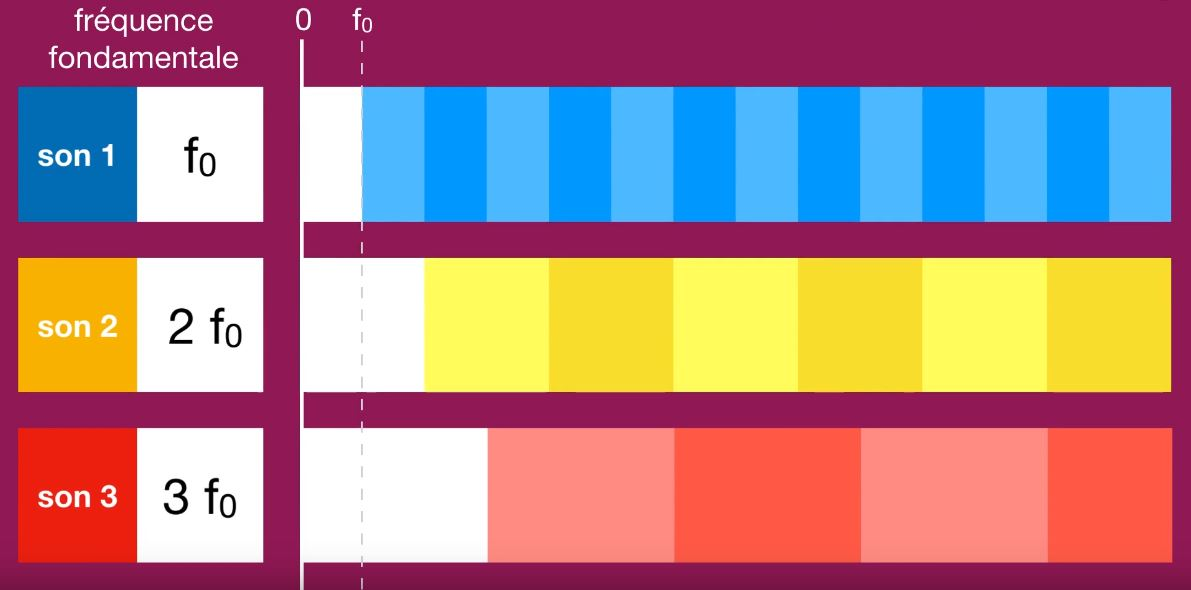
\includegraphics[width=0.6\textheight]{Notes2}
		\caption[Harmoniques et fondamentales...]{Le son 2 partage la moitié des harmoniques du son 1, le son 3 un tiers... - Source : \cite{cordierphychi_fractions_nodate}}
		\label{figure 1}
	\end{center}
\end{figure}

La construction de bonnes gammes musicales repose donc sur le principe suivant : si une note appartient à une gamme, alors les notes de fréquences doubles, triples (mais aussi moitié et tiers) de cette dernière doivent y apparaître.

\begin{definition}
	\emf{Définition 1 :} Une octave est un intervalle de fréquences de la forme $[f,2f[$.\footnote{Musicalement, on peut la définir comme l’intervalle séparant deux notes de même nom.}\\
\end{definition}

\begin{figure}[h!]
	\begin{center}
		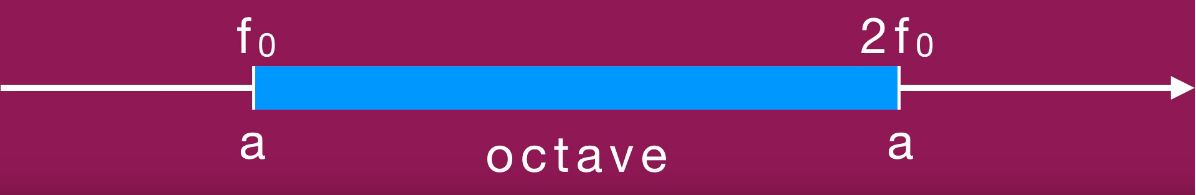
\includegraphics[width=0.6\textheight]{Octave}
		\caption[Schématisation octave]{Représentation schématique d'une octave - Source : \cite{cordierphychi_fractions_nodate}}
		\label{figure 2}
	\end{center}
\end{figure}



Afin d’obtenir une gamme complète, on transpose dans tous les autres octaves. Cela revient, d’un point de vue mathématique à répéter les notes choisies dans un octave $[f,2f[$, dans chacune des autres octaves $[2^{n}f,2^{n+1}f[$ en multipliant leur fréquence par $2^n$.
Mathématiquement parlant, ceci correspond à un sous ensemble fermé de $\mathbb{R}_{+}^{*}$, contenant une fréquence de référence, (ici appelée $f0$) et stable par multiplication et division à la fois par $2$ et $3$.\\
Mais en musique, pour faciliter écriture et transcription, il est bien plus commode de se restreindre à un nombre fini de notes. Mathématiquement, notre sous-ensemble fermé de $\mathbb{R}_{+}^{*}$  s’avère aussi être discret. \footnote{du moins dénombrable... }
\par Pour faciliter la suite des calculs, on choisit de passer en logarithme base $2$, une gamme musicale devient donc un sous-ensemble fermé discret de $\mathbb{R}$ contenant un élément de référence (que l'on suppose égal à 0) et stable par addition de $\pm1$ et $\pm \alpha$ avec $\alpha=log_{2}(3)$\\
Cependant, un ensemble A ayant ces propriétés contiendrait nécessairement le sous-groupe de $\mathbb{R}$ engendré par 1 et $\alpha$. Comme $\alpha$ est irrationnel, ce dernier est dense\footnote{En effet, le concept de densité d'un sous ensemble $A$ d'un espace $X$ suppose que pour tout point $x$ de $X$, on peut trouver un point de $A$ qui soit aussi proche de $x$ que souhaité. Grossièrement dit, cela renvoit à une forme de continuité, incompatible ici avec le caractère discret de notre gamme.}, ce qui implique que A ne saurait être discret.\\

Au final, il s’avère qu'un tel ensemble A n'existe pas.\\
L’exercice ici, tient plutôt à en chercher des approximations. Notre étude se réduira donc exclusivement aux sous-ensembles discrets de $\mathbb{R}$ stables par translation par les entiers.\
\clearpage
%cette partie la j'ai pas trop compris.

\begin{definition}
	\emf{Définition 2 :} Une gamme est partie discrète non vide de $\mathbb{R}$ stable par translation par les entiers.
\end{definition}
Une telle gamme est entièrement déterminée par son intersection avec l'intervalle $[0, 1[$, qui est un ensemble fini.

\begin{figure}[h!]
	\begin{center}
		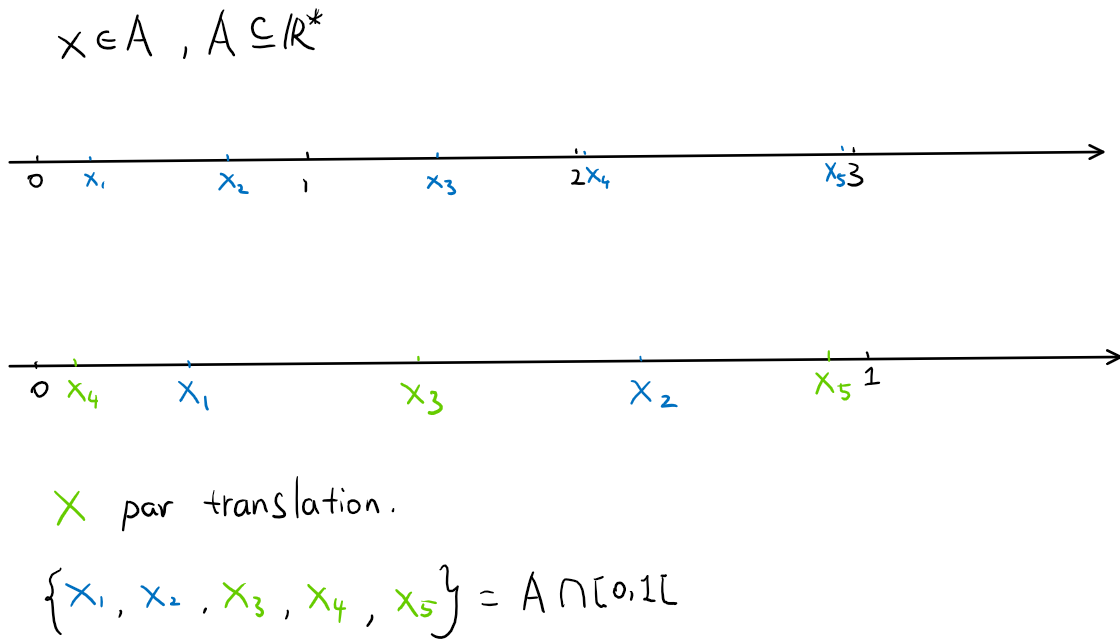
\includegraphics[width=0.7\textheight]{Inter}
		\caption[Schématisation $A\cap [0,1[$]{Représentation schématique de l'intersection de A avec $[0, 1[$ }
		\label{figure 3}
	\end{center}
\end{figure}
%here the image doesn't show , idk why...

On introduit donc la définition suivante :


%la partie défautttttttttttttttttttttttttttttttttttttttttttttttttttttttttttttttttttttttttttttttt

\begin{definition}
	\emf{Définition 3 :} La taille d'une gamme A est le cardinal de l'ensemble fini $A\cap [0,1[$. Dans la suite, on notera $q$ cette taille.\\
\end{definition}
%on a pas encore parler de 'q' ici je crois
Comment donc qualifier une gamme musicale ? Par quels moyens exprimer son caractère optimal ?
\chapter{Le défaut d’une gamme musicale}
C’est le défaut de la gamme musicale, que nous introduirons en tant que mesure de la qualité d’une gamme musicale. Définissons ce dernier comme :

\begin{definition}
\emf{Définition 4 :} Le défaut d'une gamme musicale est la quantité suivante :

\begin{equation*}
\sum_{x\in A \cap [0,1[}^{} dist(x+\alpha,A)
\end{equation*}

\end{definition}

Graphiquement, la figure \ref{figure 4} permet d'éclairer cette définition. Les accolades roses correspondent ici aux différentes distances. Le défaut est la somme de ces dernières.
 
\begin{figure}[h!]
	\begin{center}
		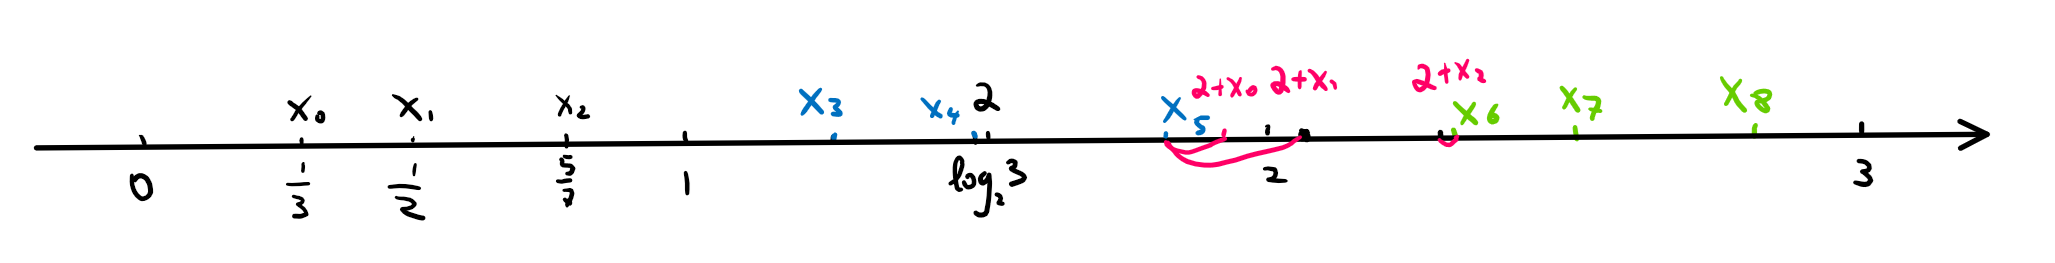
\includegraphics[width=0.7\textheight]{picture1}
		\caption[Défaut d'une gamme musicale]{Représentation schématique du défaut d'une gamme musicale}
		\label{figure 4}
	\end{center}
\end{figure}

Comment expliquer qu’une telle quantité soit utilisée en tant que mesure de la qualité d’une gamme ? Il s’agit ici de montrer que construire une bonne gamme musicale tient, mathématiquement parlant, à trouver des gammes ayant un petit défaut et une petite taille. On parle alors de gammes optimales.\\
Il n’est pas possible de minimiser simultanément ces deux paramètres (comme on le démontrera par la suite...) ; le cœur de notre problème sera donc de définir de bons compromis. La démonstration qui suit, par exemple cherche à montrer que l’on peut trouver un grand nombre de gammes à défaut optimal, si l’on se fixe une taille de gamme $q$.\\

%définition 4 dans le text d'origine .
On introduit les fonctions suivantes : $d: \mathbb{N^{*}} \longrightarrow \mathbb{R^{+}} ,d_{min} :\mathbb{N^{*}} \longrightarrow \mathbb{R^{+}} $,
$$d(q)=dist(q\alpha, \mathbb{Z})= \left|q\alpha  - s\right| ,s \in \mathbb{Z}$$
$$d_{min}(q) = min _{1 \le q' \le q} d(q') = min_{1 \le q' \le q} \left|q'\alpha - s\right| .$$

Soit A une gamme de taille q, 
$ \forall x \in \left[0,1\right[ 
\text{, on choisit } g(x)\in A$. \\
Comme $x \in [0,1[ $,  $f: x \mapsto  \{g(x)\}$  , envoie $A\cap [0,1[$ dans lui même, on parle maintenant des \textbf{itérés} de $f$, qu'on note $f^{n}$(pour $n \in \mathbb{N}$), cela veut dire que :
$$\exists q'\in \{1,2,3,.....,q\} \text{, } q'\in \mathbb{N^{*}},\exists x \in A \cap [0,1[ \text{ tel que } f^{q'}(x) = x$$



Soit $r = min (q')$, l'article \cite{caruso_application_nodate} suppose que le défaut de A soit minoré suivant l'inégalité suivante:

$$\sum_{x\in A \cap [0,1[}^{} dist(x_{r} + \alpha , A) \ge \sum_{r = 0}^{q' - 1} |x_{r} + \alpha - x_{r+1}- S_{r}|$$

En effet, on a :

$$	\sum_{x\in A \cap [0,1[}^{} |x_{r}+\alpha-\underbrace{g(x_{r})}_\text{(1)}| \ge \sum_{r = 0}^{q' - 1} |x_{r} + \alpha - x_{r+1}- S_{r}|$$

$$ \sum_{x\in A \cap [0,1[}^{} |x_{r}+\alpha-x_{r+1}- S_{r}| \ge \sum_{r = 0}^{q' - 1} |x_{r} + \alpha - x_{r+1}- S_{r}|$$


(1) : \begin{align*}
	g(x_{r}) &= \{g(x_{r})\}+S_{r}\\&=f(x_{r})+Sr\\&=x_{r+1}+S_{r}
\end{align*}

On en déduit la démonstration de la minoration du défaut par $d_{min}(q)$ :

\begin{align*}
	\sum_{x\in A \cap [0,1[}^{} dist(x_{r} + \alpha , A) &\ge \sum_{r = 0}^{q' - 1} |x_{r} + \alpha - x_{r+1}- S_{r}\\ &\ge  \left| \sum_{r = 0}^{q' - 1} (x_{r} + \alpha - x_{r+1}- S_{r})\right| \\& = \left|q'\alpha - \left(\sum_{r = 0}^{q'-1}S_{r}\right)+ \underbrace{\sum_{r = 0}^{q'-1}(x_{r}-x_{r+1})}_\text{(2)}\right| \\& = |q'\alpha-S|\\ &\ge min|q'\alpha-S|\\
	Avec: S = S_{0} + S_{1} +& S_{2} + ...+ S_{q-1}
\end{align*}
(2) : \begin{align*}
\sum_{r = 0}^{q'-1}(x_{r}-x_{r+1}) &= x_{0}-x_{1}+x_{1}-x_{2}+x_{2}-x_{3}+......+x_{q'-1}-x_{q'}\\&=x_{0}-x_{q'}\\&=0\\&\text{Avec } S = S_{0}+S_{1}+...+S_{q'-1}
\end{align*}

%donc on aurait le défaut optimal ....(à rédiger) avoir la gamme A de taille q
Par définition de $d(q’)$, il est minoré par $d(q’)$ et la proposition est bien démontrée. Cette minoration est d'autant plus intéressante, qu'elle est optimale dans le sens où pour tout $q$, on peut construire une gamme $A$ de taille $q$ et de défaut $d_{min}(q)$. Un exemple d'ensemble A ayant ces propriétés est le suivant :

\begin{equation}
A_{q}=\{r\alpha+s \text{ avec }s \in\mathbb{Z}\text{ et } 0 \leq r \le q \}
\label{equation 1}
\end{equation}\

L’exercice 1 de l'article \cite{caruso_application_nodate} de Xavier Caruso montre justement qu'en général, une gamme minimisant le défaut n'est pas unique. Nous nous dispensons ici de la démonstration par manque de temps.



%2222222222222222la partie des fractions continues22222222222222222222222
\chapter{Introduction aux fractions continues}

Supposons donc qu’a taille fixée, une gamme minimisant le défaut n’est pas unique. Cette partie a pour but d’expliquer comment les fractions continues fournissent une étude de la fonction $d_{min}$ définie précédemment. Plus généralement, il s’agit ici de monter comment elles construisent de très bonnes approximations d’un nombre réel $\alpha$. Commençons par définir de manière succincte la théorie classique des fractions continues. Ici $\alpha$ est toujours irrationnel.\\

Pour $\alpha \in \mathbb{R}\backslash\mathbb{Q}$ donc, on peut l'écrire sous la forme de sa partie entière et de sa partie décimale:
$$\alpha = a_{0}+\{\alpha_{0}\}$$
On choisit ensuite d'écrire \{$\alpha$\} sous la forme de :
$$\{\alpha\} = \frac{1}{x}$$
On a $x>1$, parce que $\alpha < 1$. De même, on peut écrire $x$ sous la même forme que $\alpha$ (partie entière + partie décimale), ce qui donne :
$$\alpha = a_{0}+ \frac{1}{a_{1}+\{\alpha_{1}\}}$$
On peut construire ainsi jusqu'à n étape, on aura alors :
$$\alpha=a_{0}+\cfrac{1}{a_{1}+\cfrac{1}{a_{2}+\cfrac{1}{a_{3}+...}}}$$
Si on enlève $\{\alpha_{n}\}$ (défini comme le quotient complet d'indice n de $\alpha$ dans l'article \cite{caruso_application_nodate} de Caruso), on retient alors $\cfrac{p_{n}}{q_{n}}$ (la n-ième réduite de $\alpha$). $p,q \in \mathbb{N}$, et donc $\cfrac{p_{n}}{q_{n}} \in \mathbb{Q} $ .

%%%%%%%%%%%%%%%%%%%%%%%%%%%%%%%%%%%%%%%%%%%%%%%%%%%%%%%%%%%%%%%%%%%%%%%%%%%%%%%%%%%%%%
\section*{ Les formules magiques des fractions continues:}
%en fait ici il y a just des propositions..... reflechis un autre nom de section peut etre.
L’article \cite{caruso_application_nodate} de Xavier Caruso fait mention d’une suite de “formules magiques” sur les fractions continues dont nous nous dispenserons de la démonstration aujourd’hui. Les voici :\\
$\forall \alpha \in \mathbb{R}\backslash\mathbb{Q}$, avec $\cfrac{p_{n}}{q_{n}}$ comme sa meilleurs approximation, on a :


$$\text{1. }p_{n}=a_{n}p_{n-1}+p_{n-2}$$
$$\text{2. }q_{n}=a_{n}p_{n-1}+q_{n-2}$$
$$\text{3. } p_{n}q_{n-1}-p_{n-1}q_{n}=(-1)^{n-1}$$
$$\text{4. }\alpha - \cfrac{p_{n}}{q_{n}} = \cfrac{(-1)^{n}}{q_{n}q_{n-1}+\alpha_{n}q_{n}^{2}}$$
$$\text{5. }\cfrac{p_{n-1}}{q_{n-1}}-\cfrac{p_{n}}{q_{n}}= \cfrac{(-1)^{n}}{q_{n}q_{n-1}}$$
$$\text{6. }\cfrac{p_{n-2}}{q_{n-2}}-\cfrac{p_{n}}{q_{n}}= \cfrac{(-1)^{n-1}a_{n}}{q_{n}q_{n-2}}$$\\

De ces formules on démontre la majoration (5) de l’article \cite{caruso_application_nodate} :\\

\begin{align*}
	\cfrac{p_{n-1}}{q_{n-1}}-\cfrac{p_{n}}{q_{n}}&= \cfrac{(-1)^{n}}{q_{n}q_{n-1}}\\
	\Rightarrow\cfrac{p_{n}}{q_{n}}-\cfrac{p_{n+1}}{q_{n+1}}&= \cfrac{(-1)^{n+1}}{q_{n+1}q_{n}}\\
	\Rightarrow\cfrac{p_{n}*q_{n+1}q_{n}}{q_{n}}-\cfrac{p_{n+1}*q_{n+1}q_{n}}{q_{n+1}}&= (-1)^{n+1}\\
	\Rightarrow p_{n}*q_{n+1}-p_{n+1}*q_{n}&= (-1)^{n+1}\\
	\Rightarrow\cfrac{p_{n}}{q_{n}}-\cfrac{p_{n+1}}{q_{n+1}}&=\cfrac{(-1)^{n+1}}{q_{n}q_{n+1}}\\
	\Rightarrow\left|\cfrac{p_{n}}{q_{n}}-\cfrac{p_{n+1}}{q_{n+1}}\right|&=\left|\cfrac{1}{q_{n}q_{n+1}}\right|\\
	\Rightarrow\left|\cfrac{p_{n}}{q_{n}}-\cfrac{p_{n+1}}{q_{n+1}}\right|&=\cfrac{1}{q_{n}q_{n+1}}
\end{align*}
Et
$$\left|\alpha-\cfrac{p_{n}}{q_{n}}\right| \le \left|\cfrac{p_{n+1}}{q_{n+1}}-\cfrac{p_{n}}{q_{n}}\right|=\cfrac{1}{q_{n}q_{n+1}}$$\\

Ce qui exprime de façon précise en quoi les réduites de $\alpha$ fournissent d'excellentes approximations : la distance à $\alpha$ est contrôlée par le carré de l'inverse du dénominateur\\

La figure \ref{figure 5} exprime visuellement cette approximation :\\

%%%%%%%%%%%%%%%%%%%%%%%%%%%%%%%
\begin{figure}[h!]
	\begin{center}
		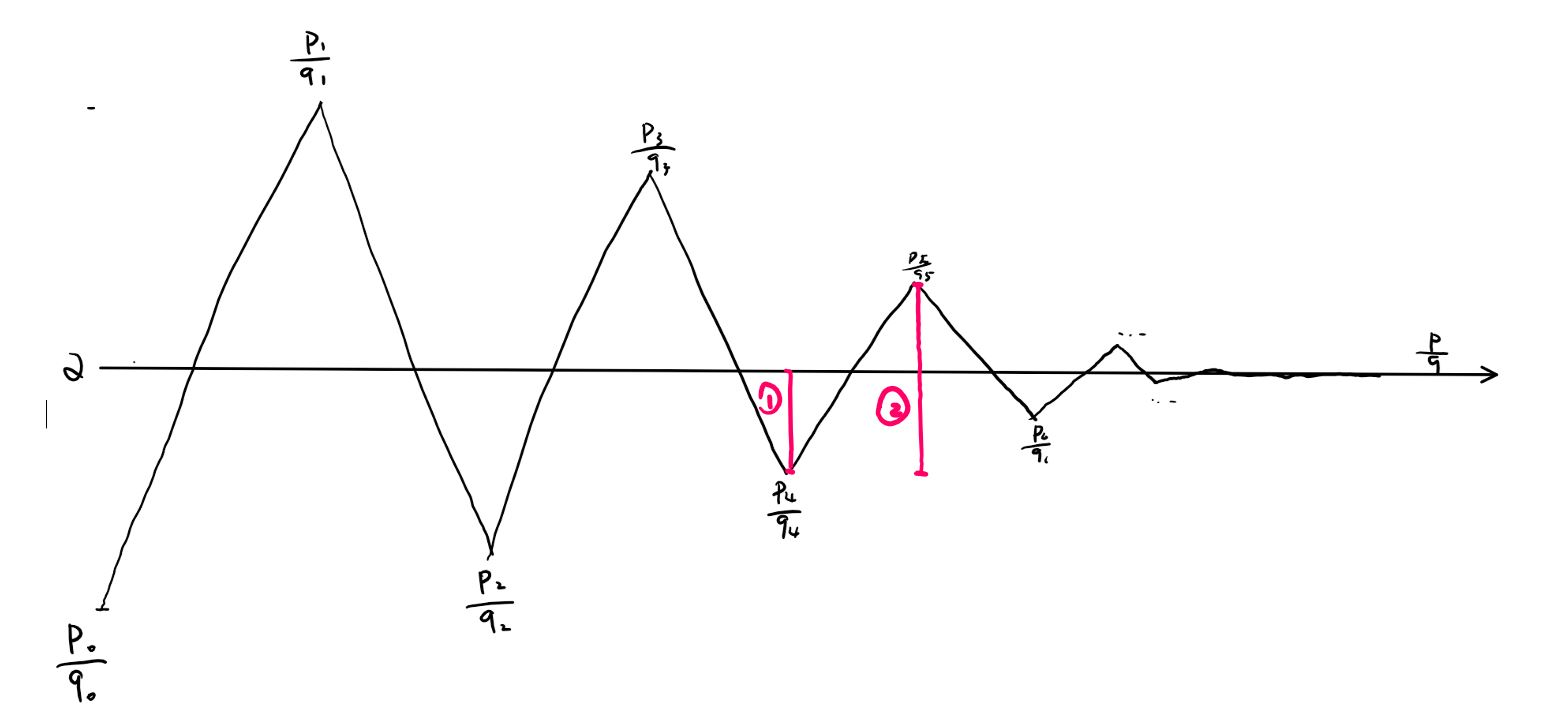
\includegraphics[width=0.8\textwidth]{SnipImage[992].jpg}
		\caption[Schématisation des réduites successives de $\alpha$ ]{Représentation schématique des réduites successives de $\alpha$ : Plus $n$ est grand mieux la réduite est une bonne approximation...}
		\label{figure 5}
	\end{center}
\end{figure}
 On peut dire que $\forall n \geq 1 $, $\cfrac{p_{n}}{q_{n}}$ sont des meilleures approximations de $\alpha$.


%gamme optimal : theoreme 10 et 11 , j'ai par encore fini
\chapter{Conséquences sur l'étude des gammes - Gammes optimales}

Nous venons de démontrer le théorème 6 de l’article \cite{caruso_application_nodate} : les réduites de $\alpha$ sont en fait ses meilleures approximations. Il s’agit ici de conclure en expliquant le lien de ce théorème avec l’étude des gammes.\\

Il est clair que la fonction $d_{min}$ est décroissante. On introduit alors les définitions suivantes :

\begin{definition}
	\emf{Définition 5:}
On dit que l'entier $q \ge 1$
est un \emph{saut} de $d_{min}$ si $q = 1$ ou si $d_{min}(q) < d_{min}(q-1)$ (dans le cas où $q > 1$).
\end{definition}

On en déduit le corolaire suivant :
\begin{definition}
	\emf{Corollaire:}
Pour un nombre irrationnel $\alpha > 0$ fixé, les sauts de la fonction $d_{min}$ sont
exactement les dénominateurs des réduites de $\alpha$.
\end{definition}

Pour une gamme $A \subset \mathbb{R}$, ensemble stable par $\pm1$ de taille :
$$\tau(A) =\#A \cap [0,1[ $$
et de défaut :
$$\delta(A) = \sum_{x \in A \cap [0,1[}^{}dist(x+\alpha,A)$$

\begin{definition}
\emf{Définition 6:}
 $A \subset \mathbb{R}$ est une gamme optimale, pour toute gamme $A'$ si: 
 $$\text{soit }\tau(A')\ge \tau(A) \text{ soit } \delta(A') \ge \delta(A)$$
 \end{definition}

 Le corollaire indique que parmi les gammes $A_q$ définies par la formule \eqref{equation 1}, les meilleures
 sont celles pour lesquelles $q$ est le dénominateur d'une réduite de $\alpha$. Car dans l'article \cite{caruso_application_nodate}, on suppose qu'à défaut fixé, ce sont elles qui ont une taille minimale. Mais rien ne le prouve, on peut supposer que ce n'est pas vrai.\\
 
 \emf{Démonstration:}\\
 
 On fixe défaut = $d_{min}(q)$, et $q$ la taille de la gamme.  Prenons $q$ un saut de $d_{min}$ et $A$ une gamme de taille $q$ mais telle que $d_{min}(q-1)\ge \delta (A)>d_{min}(q)$. Alors nous avons A optimale d'après la définition : soit $A'$ tout autre gamme, alors si $\delta(A')<\delta(A)$ nous avons nécessairement $\tau (A') \ge q = \tau (A)$ vu que $q$ est un saut. Si de telles gammes n'existent pas , il faudrait le démontrer. (chose qui n'est pas faite dans l'article \cite{caruso_application_nodate}.)\\
 
 On déduit de la remarque précédente la définition modifiée suivante :
 
 \begin{definition}
 Pour $A$ optimale et pour toute gamme $A'$:
 $$\delta(A') < \delta(A) \Rightarrow \tau(A') > \tau(A)$$
 $$\tau(A') < \tau(A) \Rightarrow \delta(A') > \delta(A)$$
 \end{definition}
 
 Si $q$ est le dénominateur de la n-ième réduite de $\alpha$, et si  $q =\tau(A) $, alors $q$ est un saut de $d_{min}$ et $\delta(A)= d_{min}(q)$. En effet pour $q'\leq q$ le saut plus proche de $q$ :
 $$d_{min}(q'-1) >d_{min}(q')=...=d_{min}(q) $$
 $$d_{min}(q) = d_{min}(q')=\delta(A_{q'})\leq \delta(A)$$
 D'après la contraposée :
 $$q' = \tau (A_{q'})\ge \tau (A) = q$$
ce qui nous dit que $q' = q$ . On peut alors démontrer par l’absurde, que $\delta(A)= d_{min}(q)$. En effet, si $\delta(A) > d_{min}(q) = \delta(A_{q})$,  la première ligne nous assure que $q = \tau (A_{q}) > \tau (A) = q$, ce qui est absurde. \\
En conclusion on a bien :
$$d_{min}(q'-1) >d_{min}(q)=\delta(A) $$
Ce qui est dit dans les premières lignes de la démonstration du théorème 11 de l'article \cite{caruso_application_nodate}, assurant ainsi d'après le corollaire que $q$ est le dénominateur d'une réduite de $\alpha$.



\clearpage
\chapter*{Conclusion}

Au cours de ce projet de mathématiques, nous avons été introduits à des notions très nouvelles, aussi abstraites que fascinantes. Nous avons réussi à montrer que si $A$ est une gamme optimale de taille $q$, alors il existe un entier $n$ tel que $q$ soit le dénominateur de la n-ième réduite de $\alpha$. Plus encore, comme l'explique notre dernière définition d'une gamme optimale, nous avons montré que défaut et taille sont deux paramètres interdépendants, qui pour dire les choses simplement, supposent que l'un ne peut diminuer sans que l'autre augmente.\\ La construction des gammes musicales repose sur la recherche de ces bons compromis, chose qui, nous en sommes conscients, n'a pas été l'objet de notre étude et nécessiterait une recherche approfondie. Par manque de temps aussi, nous n'avons pas été en mesure de montrer que les gammes optimales s'avèrent être aussi les gammes usuelles de la musique aux quatre coins du globe. La encore, un travail supplémentaire serait nécessaire.\\ Nous tenons à remercier encore une fois M. Andrei Bengus-Lasnier pour avoir accepté de nous aider à la résolution de l'exercice 1 de l'article \cite{caruso_application_nodate}, pour ses explications du théorème 11, et M. Yves Capdeboscq pour son encadrement, sa patience et sa bienveillance.

\clearpage
\listoffigures
\printbibliography


\end{document}          
